\documentclass[../main]{subfiles}
\begin{document}

\chapter{任意信号发生器}%
\label{cha:ramgen}

\section{实验要求}%
\label{sec:\arabic{chapter}requirement}

\begin{Exercise}
  独立完成项目编译、链接、调试的全过程。
\end{Exercise}

\begin{Answer}
  已完成。
\end{Answer}

\begin{Exercise}
  记录实验中子程序包括主程序的入口实际地址,与 memory 比较,指出分别位于什
  么类型的存储器中。
\end{Exercise}

\begin{Answer}
  \begin{itemize}
    \item 由 CCS 的 Expression 可知入口实际地址。
    \item 由入口实际地址和 \url{code/LAB10/Debug/LAB10.map} 的 MEMORY
      CONFIGURATION 可知存储空间。
    \item 由存储空间和 \url{https://www.ti.com.cn/cn/lit/gpn/tms320f28335}
      156 页的图 6--23 可知物理存储块名称。
    \item 由物理存储块可知存储器类型。
  \end{itemize}
  见表~\ref{tab:entry}。
\end{Answer}

\begin{table}[htbp]
  \centering
  \caption{入口}%
  \label{tab:entry}
  \csvautobooktabular[respect all]{tables/entry.csv}
\end{table}

\begin{Exercise}
  指出波形数据保存的空间地址,并以图形方式显示线性调频信号的波形,并保存,附
  在实验报告中。
\end{Exercise}

\begin{Answer}
  由 CCS 的 Expression 可知波形数据地址为 0xF000 。原代码的公式
  式~\ref{eq:sine}为正弦信号,不符合线性调频信号的公式式~\ref{eq:k}。根据约束
  条件式~\ref{eq:t}求出式~\ref{eq:ta}代入式~\ref{eq:k}得到式~\ref{eq:lfm}。根
  据式~\ref{eq:lfm}修改代码如程序~\ref{lst:lfm},结果见图~\ref{fig:lfm}。
  仿真代码见程序~\ref{lst:plot}第一段。
\end{Answer}

\begin{align}
  \label{eq:sine}
  x\lbrack i\rbrack = & \sin 2\pi \frac{i}{1024} & i = 0..1024\\
  \label{eq:k}
  y\lbrack i\rbrack = & \cos 39062 \pi {t\lbrack i\rbrack}^2 & i = 0..1024\\
  \label{eq:t}
  \lvert t\lbrack i\rbrack\rvert \leqslant & 0.0128 & i = 0..1024\\
  \label{eq:ta}
  t\lbrack i\rbrack = & \frac{i - 512}{1024}\frac{16}{625} & i = 0..1024\\
  \label{eq:lfm}
  y\lbrack i\rbrack = & \cos 39062 \pi {\left(\frac{i - 512}{1024}
  \frac{16}{625}\right)}^2 & i = 0..1024
\end{align}

\begin{listing}[htbp]
  \centering
\begin{langPyOne}[c][firstnumber = 68]{code/LAB10/main.c}
for(i=0;i<1024;i++)
	*(RamAddr+i) = (int)(cos(39062*Pi*(i - 512)/1024*16/625*(i - 512)/1024*16/625)*4096);
\end{langPyOne}
  \caption{线性调频代码}%
  \label{lst:lfm}
\end{listing}

\begin{figure}[htbp]
  \centering
  \begin{subfigure}[htbp]{0.45\linewidth}
    \centering
    \includegraphics[
      width = \linewidth,
    ]{figures/lfm.pdf}
    \caption{仿真}%
    \label{fig:lfm/simulation}
  \end{subfigure}
  \quad
  \begin{subfigure}[htbp]{0.45\linewidth}
    \centering
    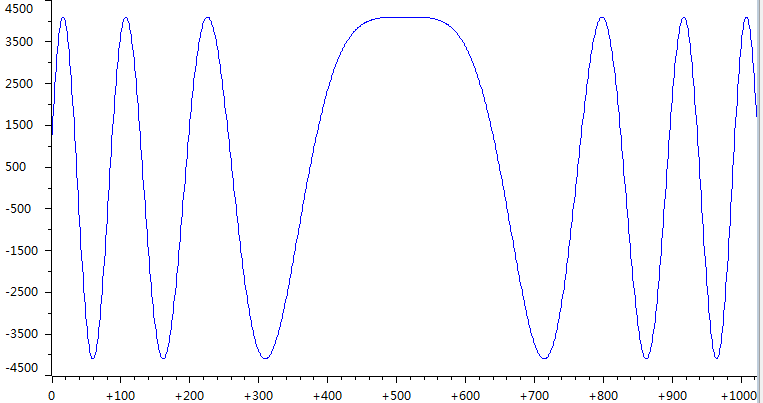
\includegraphics[
      width = \linewidth,
    ]{images/lfm_plot.png}
    \caption{CCS 绘图}%
    \label{fig:lfm/plot}
  \end{subfigure}

  \begin{subfigure}[htbp]{0.45\linewidth}
    \centering
    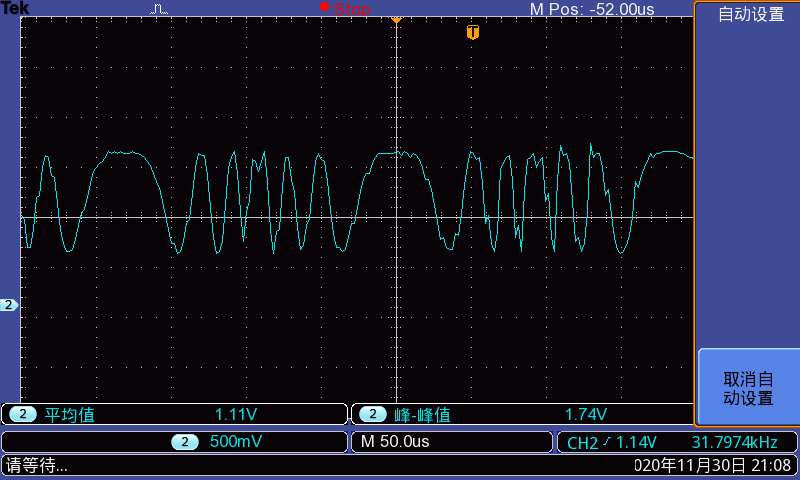
\includegraphics[
      width = \linewidth,
    ]{images/lfm_watch.png}
    \caption{观测}%
    \label{fig:lfm/watch}
  \end{subfigure}
  \caption{线性调频信号波形}%
  \label{fig:lfm}
\end{figure}

\begin{listing}
  \centering
  \langCVfile[matlab][][matlab]{figures/lfm.m}{figures/lfm.m}
  \caption{仿真代码}%
  \label{lst:plot}
\end{listing}

\begin{Exercise}
  比较波形数据保存的不同存储空间区域(DPS 内部 RAM 和外扩 SRAM),对系统实现
  的影响。
\end{Exercise}

\begin{Answer}
  \begin{description}
    \item[内部 RAM]成本高,采用片内总线,读写速率快;
    \item[外扩 SRAM]成本低,采用系统总线,读写速率慢。
  \end{description}
\end{Answer}

\section{实验思考}%
\label{sec:\arabic{chapter}thought}

\begin{Exercise}
  打开工程的 .map 文件,与实验 9 比较,指出编译产生的段有哪些区别。
\end{Exercise}

\begin{Answer}
  \begin{itemize}
    \item 由 \url{code/LAB9/Debug/LAB9.map} 和
      \url{code/LAB10/Debug/LAB10.map} 可知段的地址。
  \end{itemize}
  见表~\ref{tab:diff}。
\end{Answer}

\begin{table}[htbp]
  \centering
  \caption{区别}%
  \label{tab:diff}
  \tiny
  \csvautobooktabular[respect percent]{tables/diff.csv}
\end{table}

\begin{Exercise}
  在保持源文件功能正确的前提下,仅修改 .cmd 配置命令文件,改变段的地址分配,链
  接工程后,执行程序,如果出现错误,思考原因。
\end{Exercise}

\begin{Answer}
  错误的原因可能有:

  \begin{itemize}
    \item 由程序~\ref{lst:volatile} ,一些被明确声明的指针地址的段不存在。
    \item 段与段的地址发生重叠。
  \end{itemize}
\end{Answer}

\begin{listing}[htbp]
  \centering
\begin{windark}{cmd}
> grep 'volatile' -rn code/LAB10/main.c
22:volatile int *RamAddr = (volatile int *) 0x00F000;
24://volatile int *zone7Addr = (volatile int *) 0x20FC10;
26:volatile Uint16  *Da_freq      = (Uint16 * )0x201100;
28:volatile Uint16  *SPI_Reset   = (Uint16 * )0x202C00;
Binary file code/LAB10/main.c matches
\end{windark}
  \caption{搜索}%
  \label{lst:volatile}
\end{listing}

\begin{Exercise}[label = ex:dds]
  在不修改波形数值计算子模块前提下,即保持波形数值表中的数据,依照 DDS 原理,
  修改程序,调整线性调频信号的输出周期。
\end{Exercise}

\begin{Answer}
  DDS 原理等价为:已知式~\ref{eq:sine}和式~\ref{eq:lfm},求能满足
  式~\ref{eq:q} 的解式~\ref{eq:a}。

  根据式~\ref{eq:a}修改代码如程序~\ref{lst:dds}\footnote{数组 out 即为
  $y\lbrack i\rbrack$,因为 Da\_out 不是数组,无法进行 CCS 绘图。},仿真、
  CCS 绘图、观测结果与图~\ref{fig:lfm}基本相同\footnote{因为数组索引只能是整
  数,所以在程序~\ref{lst:dds}中取整会导致精度误差,但从图像上可忽略不计。
}。仿真代码见程序~\ref{lst:plot}第二段。
\end{Answer}

\begin{align}
  \label{eq:q}
  y\lbrack i\rbrack = & x\lbrack j\lbrack i\rbrack\rbrack & i = 0..1024\\
  \label{eq:a}
  y\lbrack i\rbrack = & x\lbrack\lfloor{(i - 512)}^2/80 + 256\rfloor \%
  1024\rbrack & i = 0..1024
\end{align}

\begin{listing}[htbp]
  \centering
\begin{langPyOne}[c][firstnumber = 75]{code/LAB10/main.c}
    	for(i=0;i<1024;i++)
    	{
    		out[i]=*(RamAddr+(int)((i - 512)*(i - 512)/80 + 256)%1024);
    		*Da_out = (unsigned int)(out[i]<<4)+ 0x8000;//左移4位
    		//*Da_out = (unsigned int)((*(RamAddr+1*i))<<3);
    	}
\end{langPyOne}
  \caption{DDS 原理代码}%
  \label{lst:dds}
\end{listing}

\section{实验总结}%
\label{sec:\arabic{chapter}conclusion}

该实验的问题~\ref{ex:dds}有一定难度,求式~\ref{eq:a}有一定计算量,花了一定时
间在程序~\ref{lst:plot}。

一些需要注意的地方:

\begin{itemize}
  \item 如果整型变量的符号类型错误,就会出现有符号型转换为无符号型的情况,导
    致图~\ref{fig:lfm/watch}沿着横轴翻转。
\end{itemize}

\end{document}

